\chapter{User Study}

\section{Objective}
\section{Objective}
The objective of the study was to build the posture classification model, analyse the posture behaviour patterns in two scenarios, and investigate the perspectives to the issues related to the design of the system.

\section{Method}
\subsection{Posture Measurement}
The study had three sections. In the first section, the postures would be measured. A proper posture would be assessed in the beginning of this section to set the baseline. Following, The participants would be asked to have a particular posture type, such as slouch, given a degree of freedom for them to interpret the posture by their usual way. The step would be repeated for four times until the target postures including cross-legs, slouch, lower back not supported, and stationary were measured. Each measurement would last for 3 minutes, but the participant would not be informed in advance. They were encouraged to relax and do their chosen relaxing activity, such as watching TV or surfing the internet on their mobile devices. This aims at simulating the normal conditions that the participants engaged in the VTDs related activities with the target unhealthy postures.

A Kinect would be placed right in front of where the participants sit to record the positions of 25 joints in the body. A digital video (DV) would videotape from the side. Each participant would be asked to have all postures in different order to balance a potential carry-over effect. The balance method follows the design of Latin square. The participants would be randomly assigned into four groups and their postures would be observed following the order presented in Table 4.1. Generally, there would be the rest time for one minute between two trials, which could be extended if needed. A Likert five-point scale would be applied during the rest time to get the subjective information about the degree of relax and the degree of shoulder, neck, and spine comfort (namely, discomfort) the participants felt when they were having the tested posture. If a participant reported discomfort in any part of the body due to the posture, a following question would be asked to clarify the sense by giving multiple choices including pain, soreness, and tightness. The subjective judgement for current viewing height and the degree of comfort for current viewing height would also be investigated as the criteria for a low-viewing height posture could be relatively vague. 

\begin{table}[ht]
\centering
\begin{tabular}{c c c c c}
Group&Posture1&Posture2&Posture3&Posture4 \\
\hline
Group1&leg crossed&lower back&slouch&stationary \\
Group2&lower back&leg crossed&stationary&slouch \\
Group3&slouch&stationary&leg crossed&stationary \\
Group4&stationary&slouch&lower back&leg crossed \\ [1ex]
\hline
\end{tabular}
\label{table:nonlin}
\caption{Order of the posture measurement for different groups}
\end{table}

\subsection{Scenario Observation}
In the second section, the behaviour pattern the participants had when they were engaging in the VDT activities would be observed. The participants were randomly assigned into two groups. Participants in the first group would watch their chosen videos on TV, and those in the other group would use their own mobile device freely. The activities for the two groups all lasted for 15 minutes. Some further information would be investigated after the activities, which included the subjective cognition for the degree of relax when doing the prior activity, and the similarity between the behaviours of doing the activity in the lab settings and doing the activity in real life.The data which had a low similarity score would be discarded as the data could not reflect the behaviour pattern for the users in real life. The valid data filtered by the question would be used to analyse the frequency of different target postures. The priority among the target postures for being feedbacked would be decided by the occurrence rate and the degree of discomfort for each posture.

\subsection{Interview}
The aims of the section was to gather more information about the posture pattern for each participant by an interview. The participant would be asked about their:

\begin{enumerate}
\item past musculoskeletal disorder history
\item musculoskeletal discomfort in the past three months and the subjective explanation for it
\item subjective evaluation to the overall posture pattern of themselves
\item awareness of bad postures with respect to the timing and the extend
\item effort had been made to improve postures with respect to the methods, durations, and results
\item reasons to improve the postures
\item preference for different feedback methods subject to a home environment.
\item belief for the effective extent of different feedback methods subject to a home environment.
\item preference for different feedback channel subject to a home environment.
\item belief for the effective extent of different feedback channel subject to a home environment.
\end{enumerate}

\section{Participant}
12 university students aged between 20 and 30, body height between 156 to 172 cm (average = 164.3), with no significant musculoskeletal disorder history.

\section{Material}

\subsection{Experimental apparatus and resources}
The following materials were used to measure the posture, record the procedure, facilitate the scenario observation and the interview, and ask the subjective feelings and perspectives of the participants.

\begin{itemize}
 \item A Microsoft Kinect
 \item A digital video
 \item A television
 \item Tokens
 \item Likert five-point scales:
  \begin{itemize}
   \item degree of relax
   \item degree of neck comfort
   \item degree of shoulder comfort
   \item degree of spine comfort
   \item degree of current viewing height
   \item degree of the similarity between the behaviours in the test condition and normal condition
  \end{itemize}
\end{itemize}

\subsection{Documents for ethics approval}

The ethical considerations of the study were approved by The University Teaching and Research Ethics Committee. The approval letter for the study could be seen in Appendix H. The following sheets were given to the participants to protect their right and ensure they understood the study.

\begin{itemize}
\item Participant Information Sheet (See Appendix~\ref{appendix:information_sheet})
\item Participant Consent Sheet (See Appendix~\ref{appendix:consent_form})
\item Participant Debriefing Form (See Appendix~\ref{appendix:debrief_form})
\end{itemize}

\section{Procedure}
The instructions of the researcher through the study would be standardised to decrease the bias (See Appendix~\ref{appendix:instructions}). At the beginning, the researcher would explain the objectives and the outline of the study and then inform the rights of the participants before asking them to read and sign on the consent form. There should be only one participant to take the experiment at one time to avoid potential confounding variables related to their interaction. A set of postures would be measured in a specific order in the first section of the study. Likert scales would be applied between the measurements of two postures. The behaviour pattern for engaging in an VTD related activity would be recorded in the second section. The subjective cognition for degrees of relax when doing the test activity as well as the similarity between behaviours in the test condition and real-life conditions were also investigated. In the last section, an interview was carried out to understand more information about the posture and posture improvement associated perspectives of the participants before the debriefing procedure. The whole study would last for approximately an hour.

\section{Analysis}
The participants rated their posture appropriateness between 2 to 4 (average = 2.92, standard deviation = 0.79) on a Likert 5-point scale. However, even though the participants believed their posture behaviour are not bad in general, there still are 66 percent of the participants who experienced musculoskeletal discomfort, including back, waist and shoulder soreness, neck and shoulder tightness, and neck, shoulder, spine, and back pain, in the past three months. 88 percent of them contributed at least part of the discomfort to bad postures, in particular to the behaviours related to using computer, such as prolonged sitting when working on the laptop.

As for the bad posture awareness, only 25 percent of the participants reported that they would notice they were having a bad posture before feeling any discomfort. 58.33 percent of the participants said they would find they are having posture when they have experienced the soreness, tightness, pain, or numbness caused by it. 16.67 percent of the participants even would not find their current bad postures until they are about to change to another posture. However, the participants gave an average 3.08 for their bad posture awareness (standard deviation = 0.90)on the 5-point scale. The fact might indicate that they tend to overestimate their awareness on bad postures, but current feedback system could be helpful for improving the awareness.

\subsection{Posture Modelling}
There are some formula rendered by the observation of the target postures. The parameters of the formula would be defined using the data collected from the section one : Posture Measurement. The data from the posture measurement procedure would be used to fit the model and find the optimised parameters. The optimised formula for one posture is defined as a formula which has the highest hit rate among the data of the target posture, and the lowest false alarm rate among the data of the proper posture.

\begin{enumerate}
  \item leg crossed (would use the pictures of the participants instead)
  \begin{itemize}
    \item type 1 \hfill \\
    \[| Y of Left Feet - Y of Right Feet | > a\]
    \[AND\]
    \[ Distance( PositionOf Left Knee - PositionOf Right Knee) > b\]

    \begin{figure}[h]
    \centering
      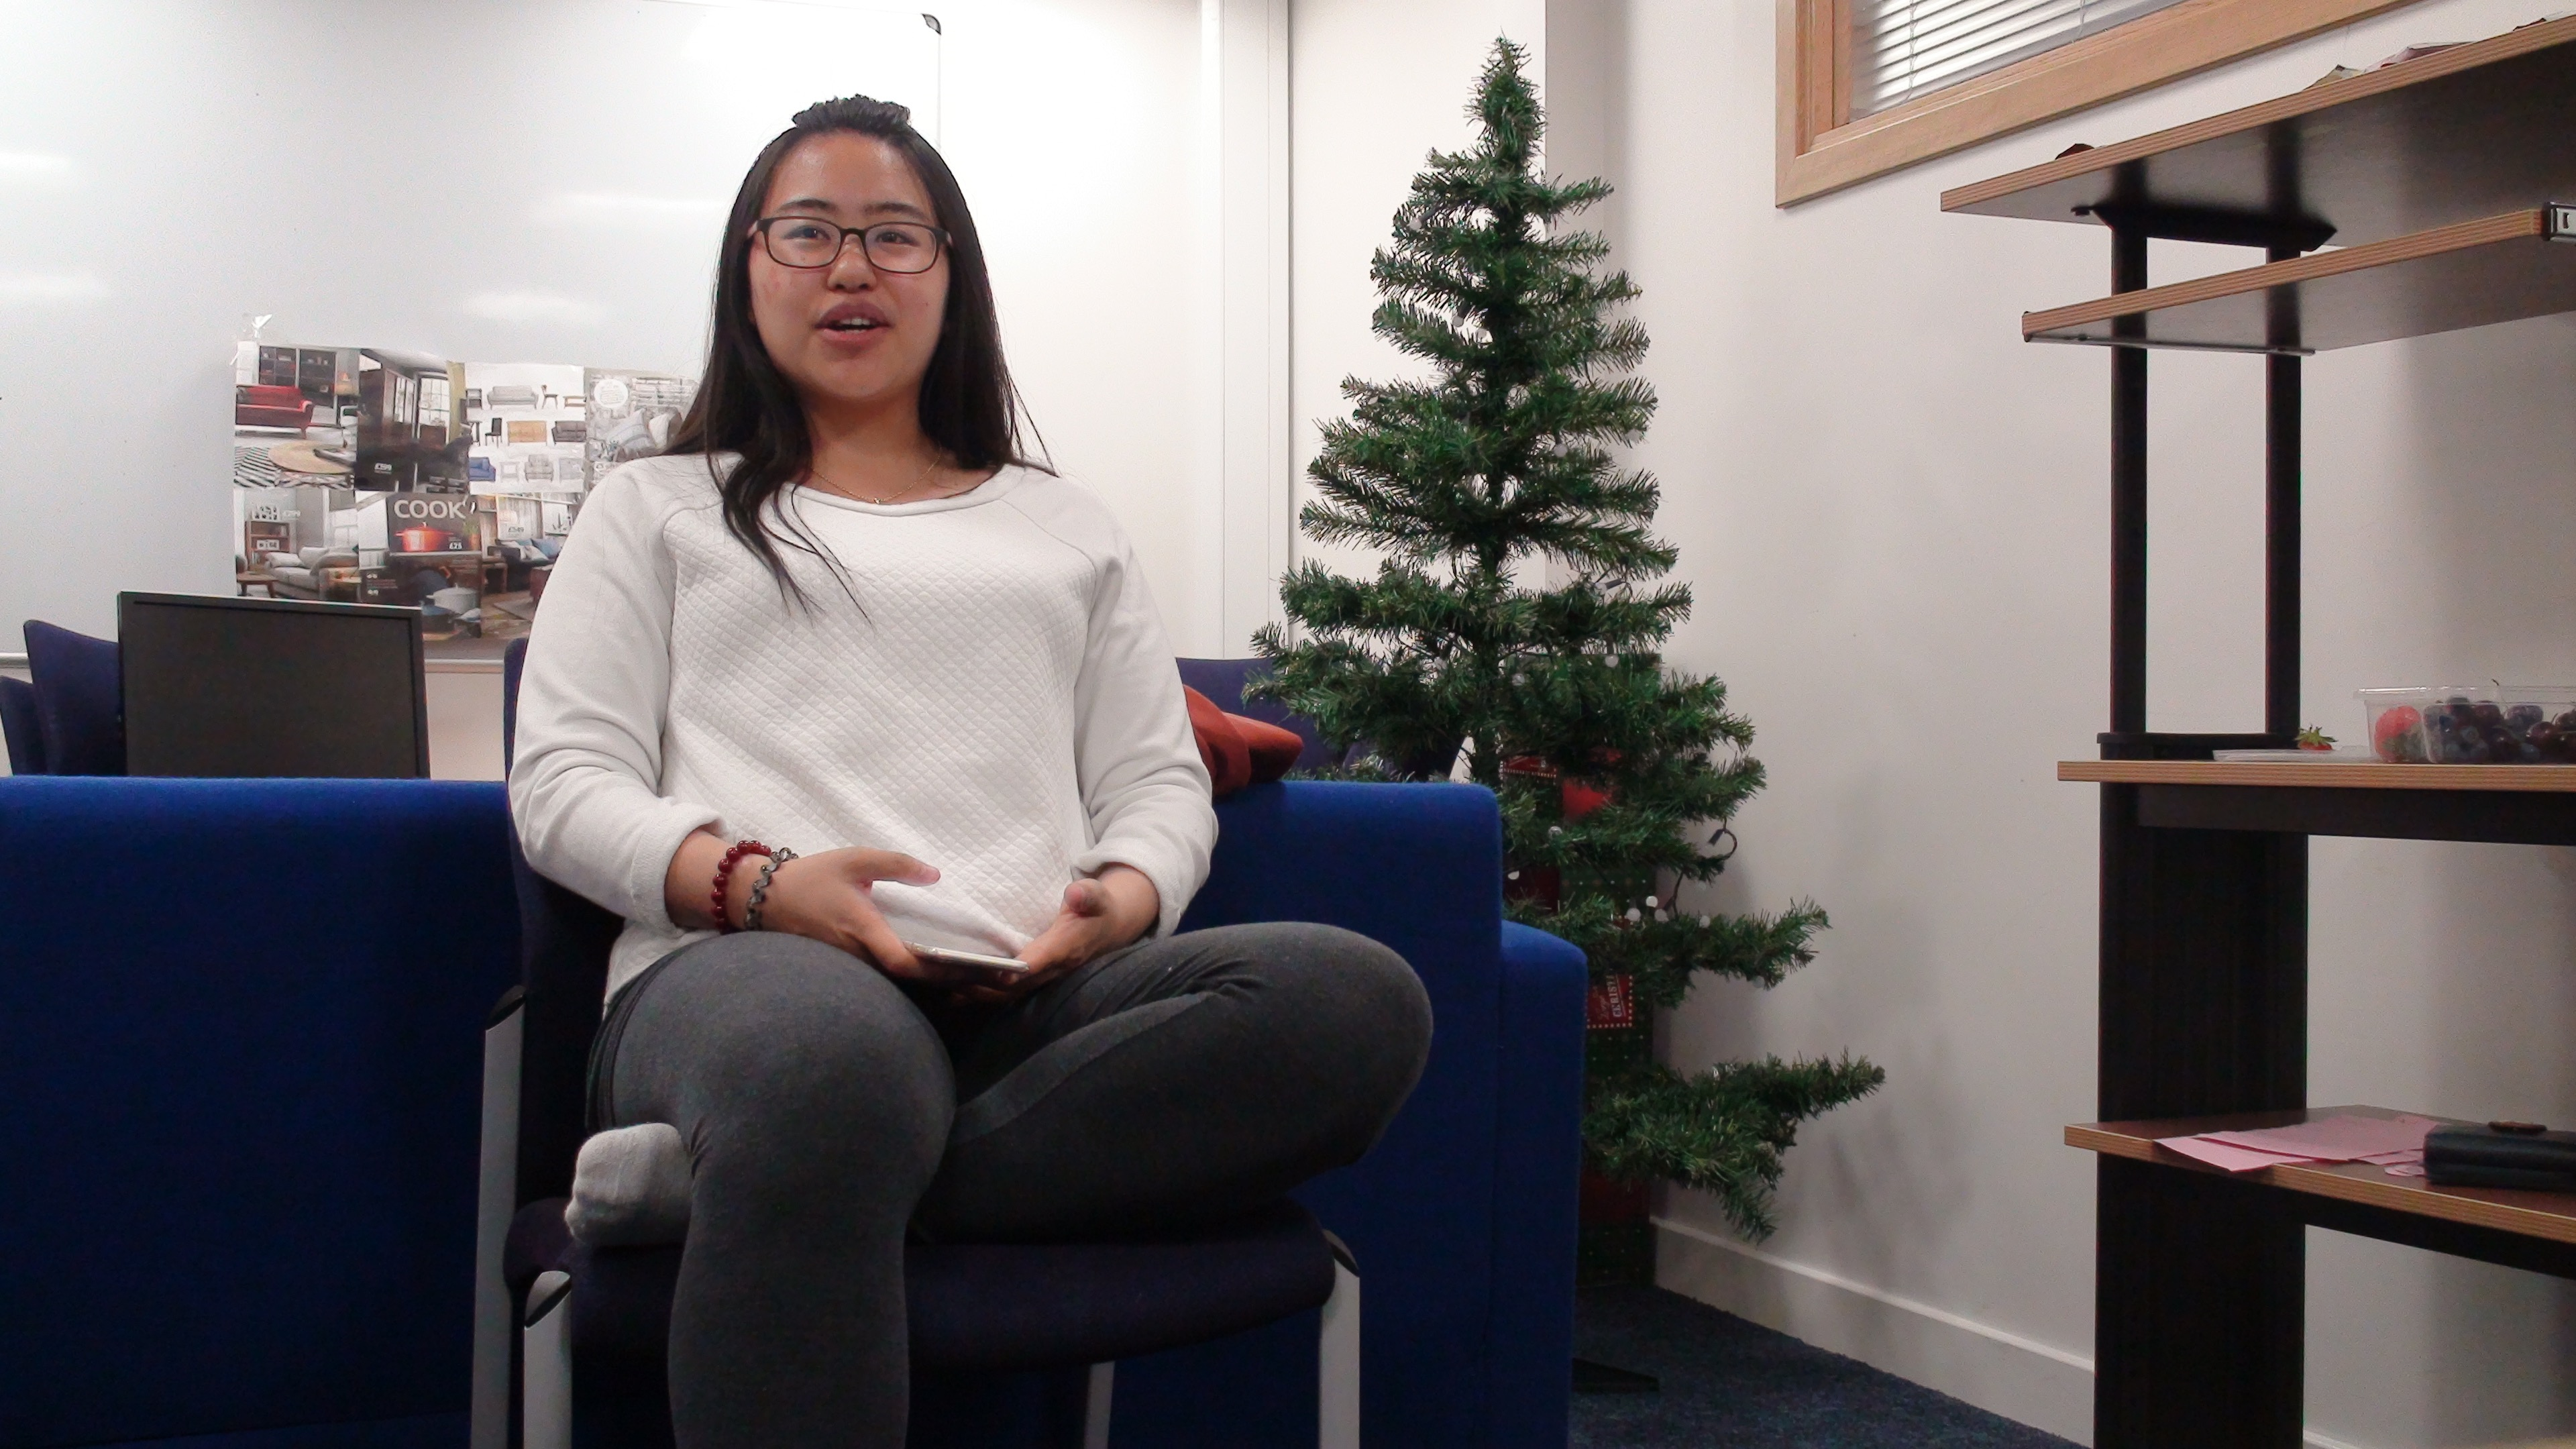
\includegraphics[width=0.5\textwidth]{figs/c1}
    \caption{Leg-Crossed Type 1}
    \end{figure}

    \item type 2 \hfill \\
    \[ ( X of Left Feet - X of Right Feet)* (X of Left Shoulder - X of Right Shoulder) < 0\]
    \[ OR\]
    \[ ( Z of Left Feet - Z of Right Feet)* (Z of Left Shoulder - Z of Right Shoulder) < 0\]\\

    \begin{figure}[h]
    \centering
      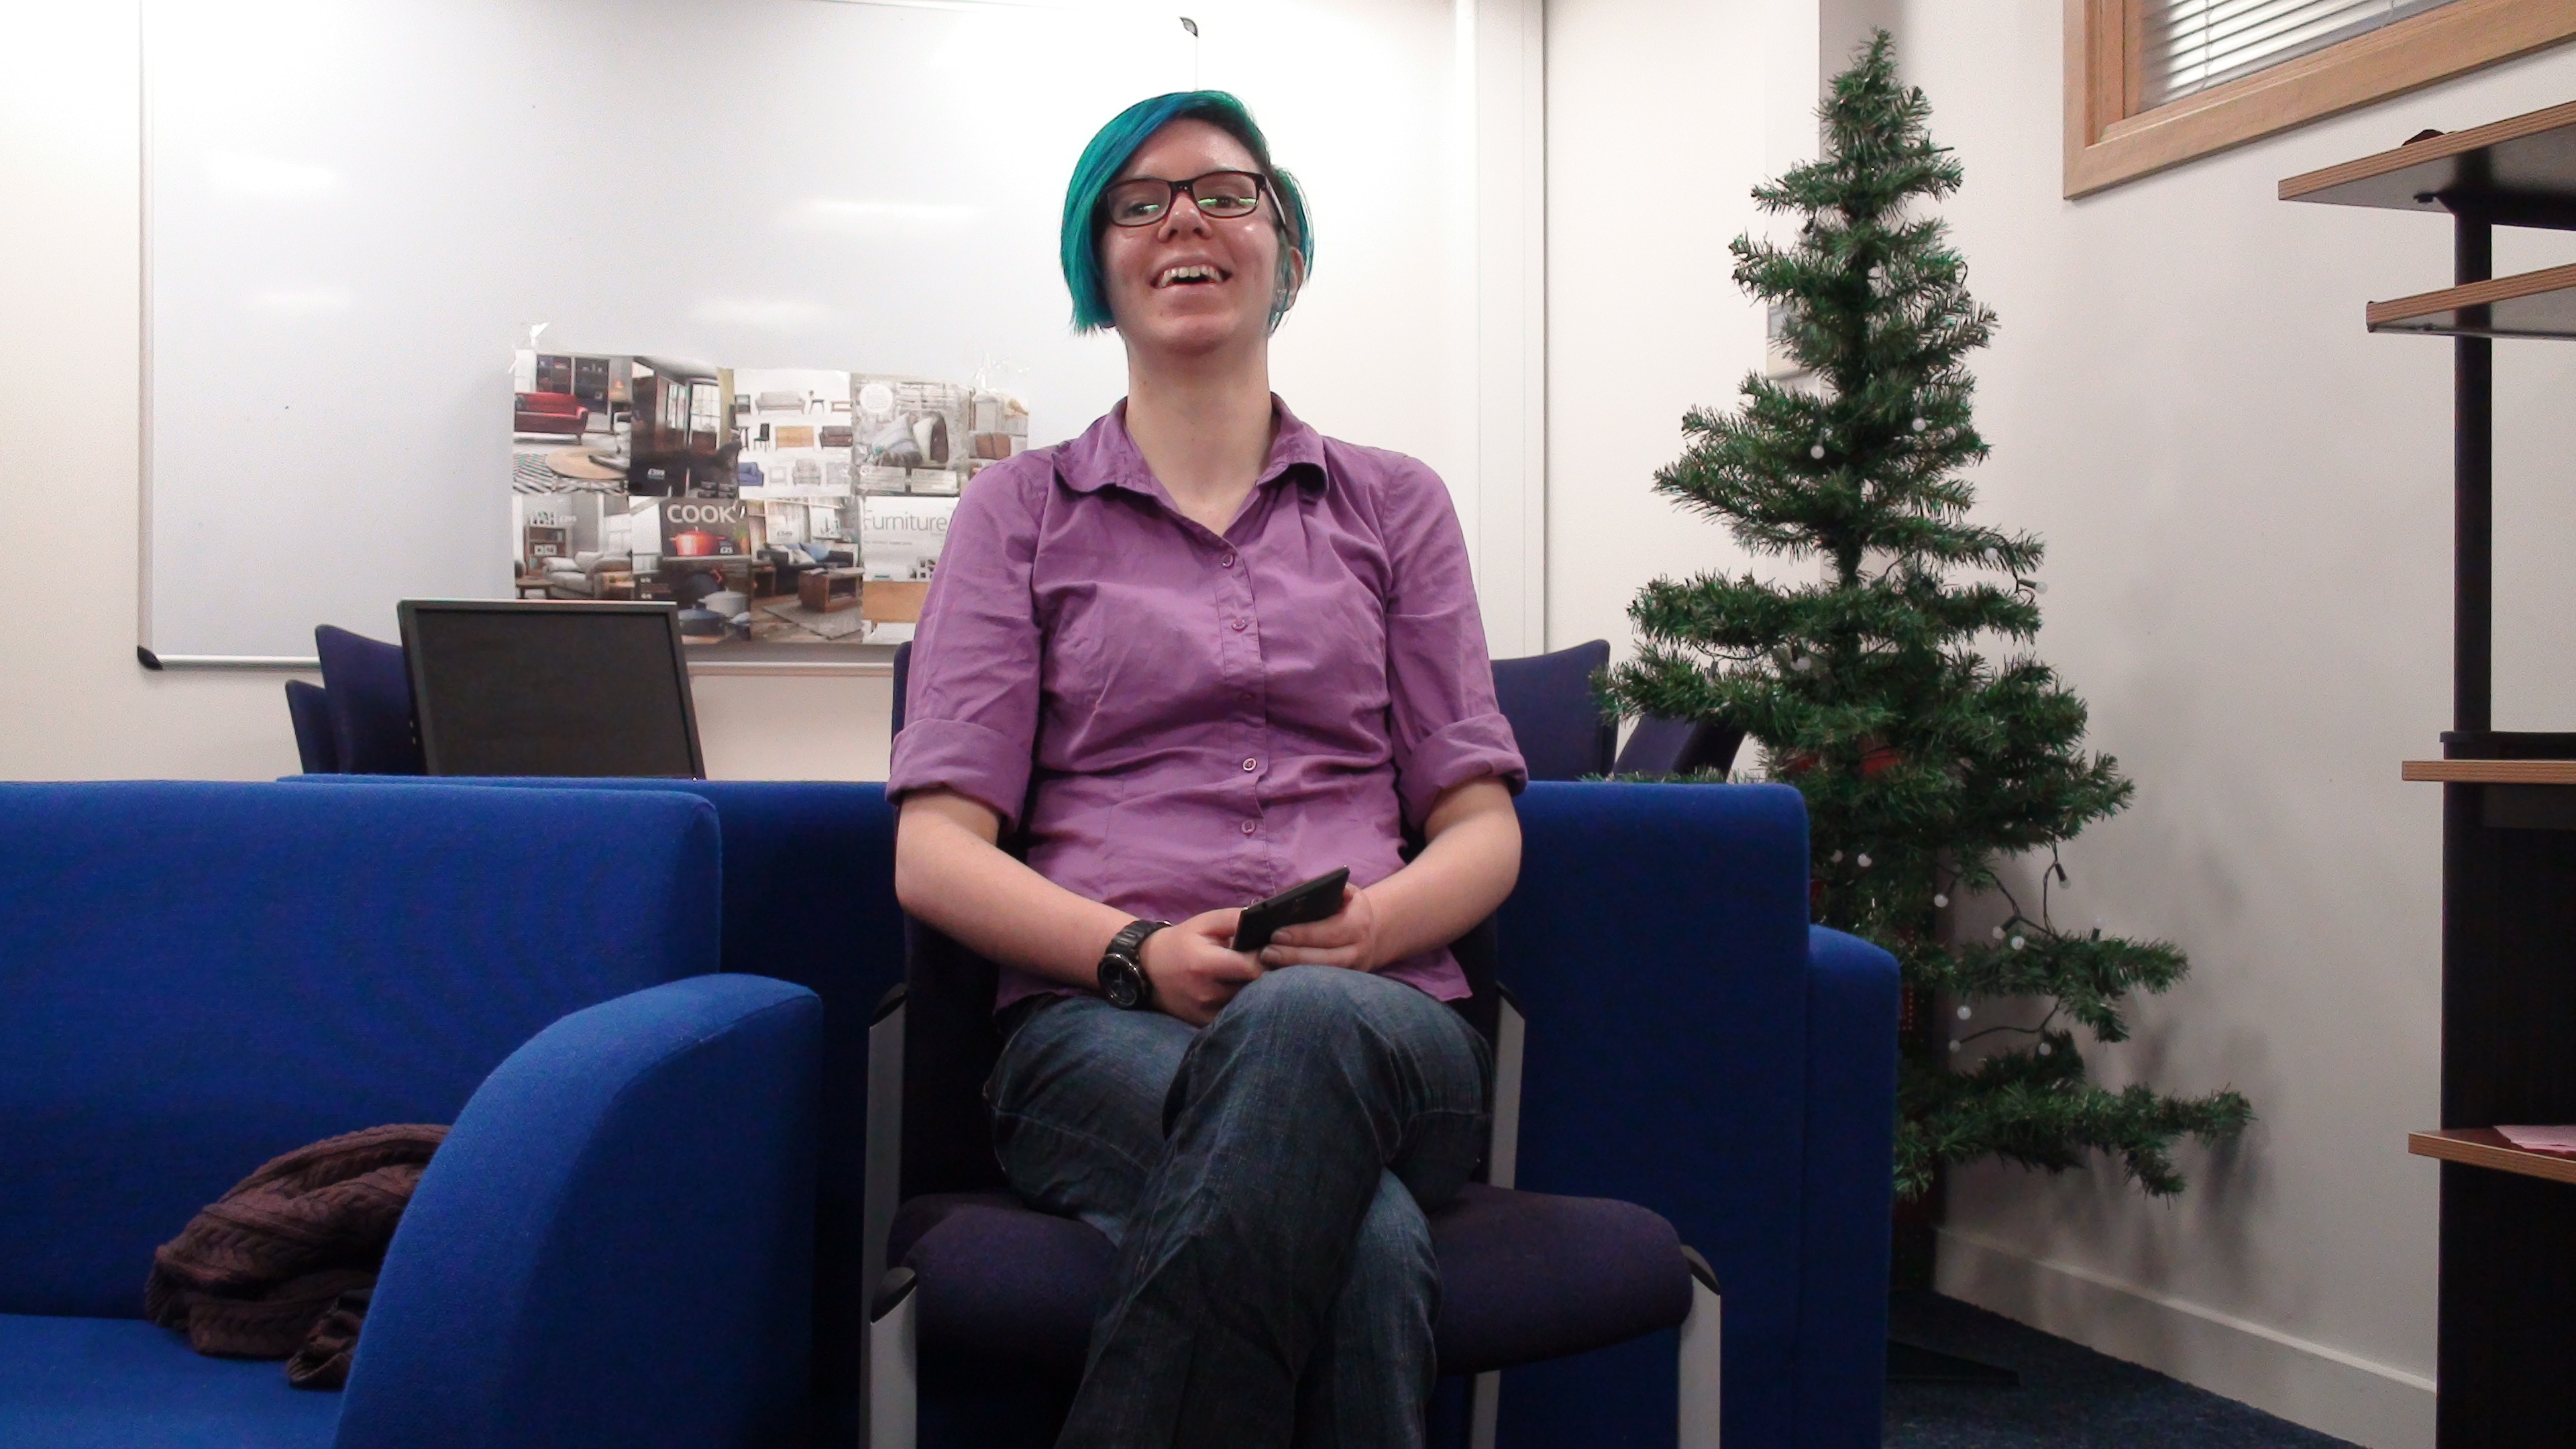
\includegraphics[width=0.5\textwidth]{figs/c2}
    \caption{Leg-Crossed Type 2}
    \end{figure}

    \item type 3 \hfill \\
    \[( ( X of Left Feet - X of Right Feet)* (X of Left knee - X of Right knee) < 0\]
    \[OR\]
    \[ ( Z of Left Feet - Z of Right Feet)* (Z of Left knee - Z of Right knee) < 0)\]
    \[AND\]
    \[ Distance(PositionOf Left Knee - PositionOf Right Knee)> c\]

    \begin{figure}[h]
    \centering
      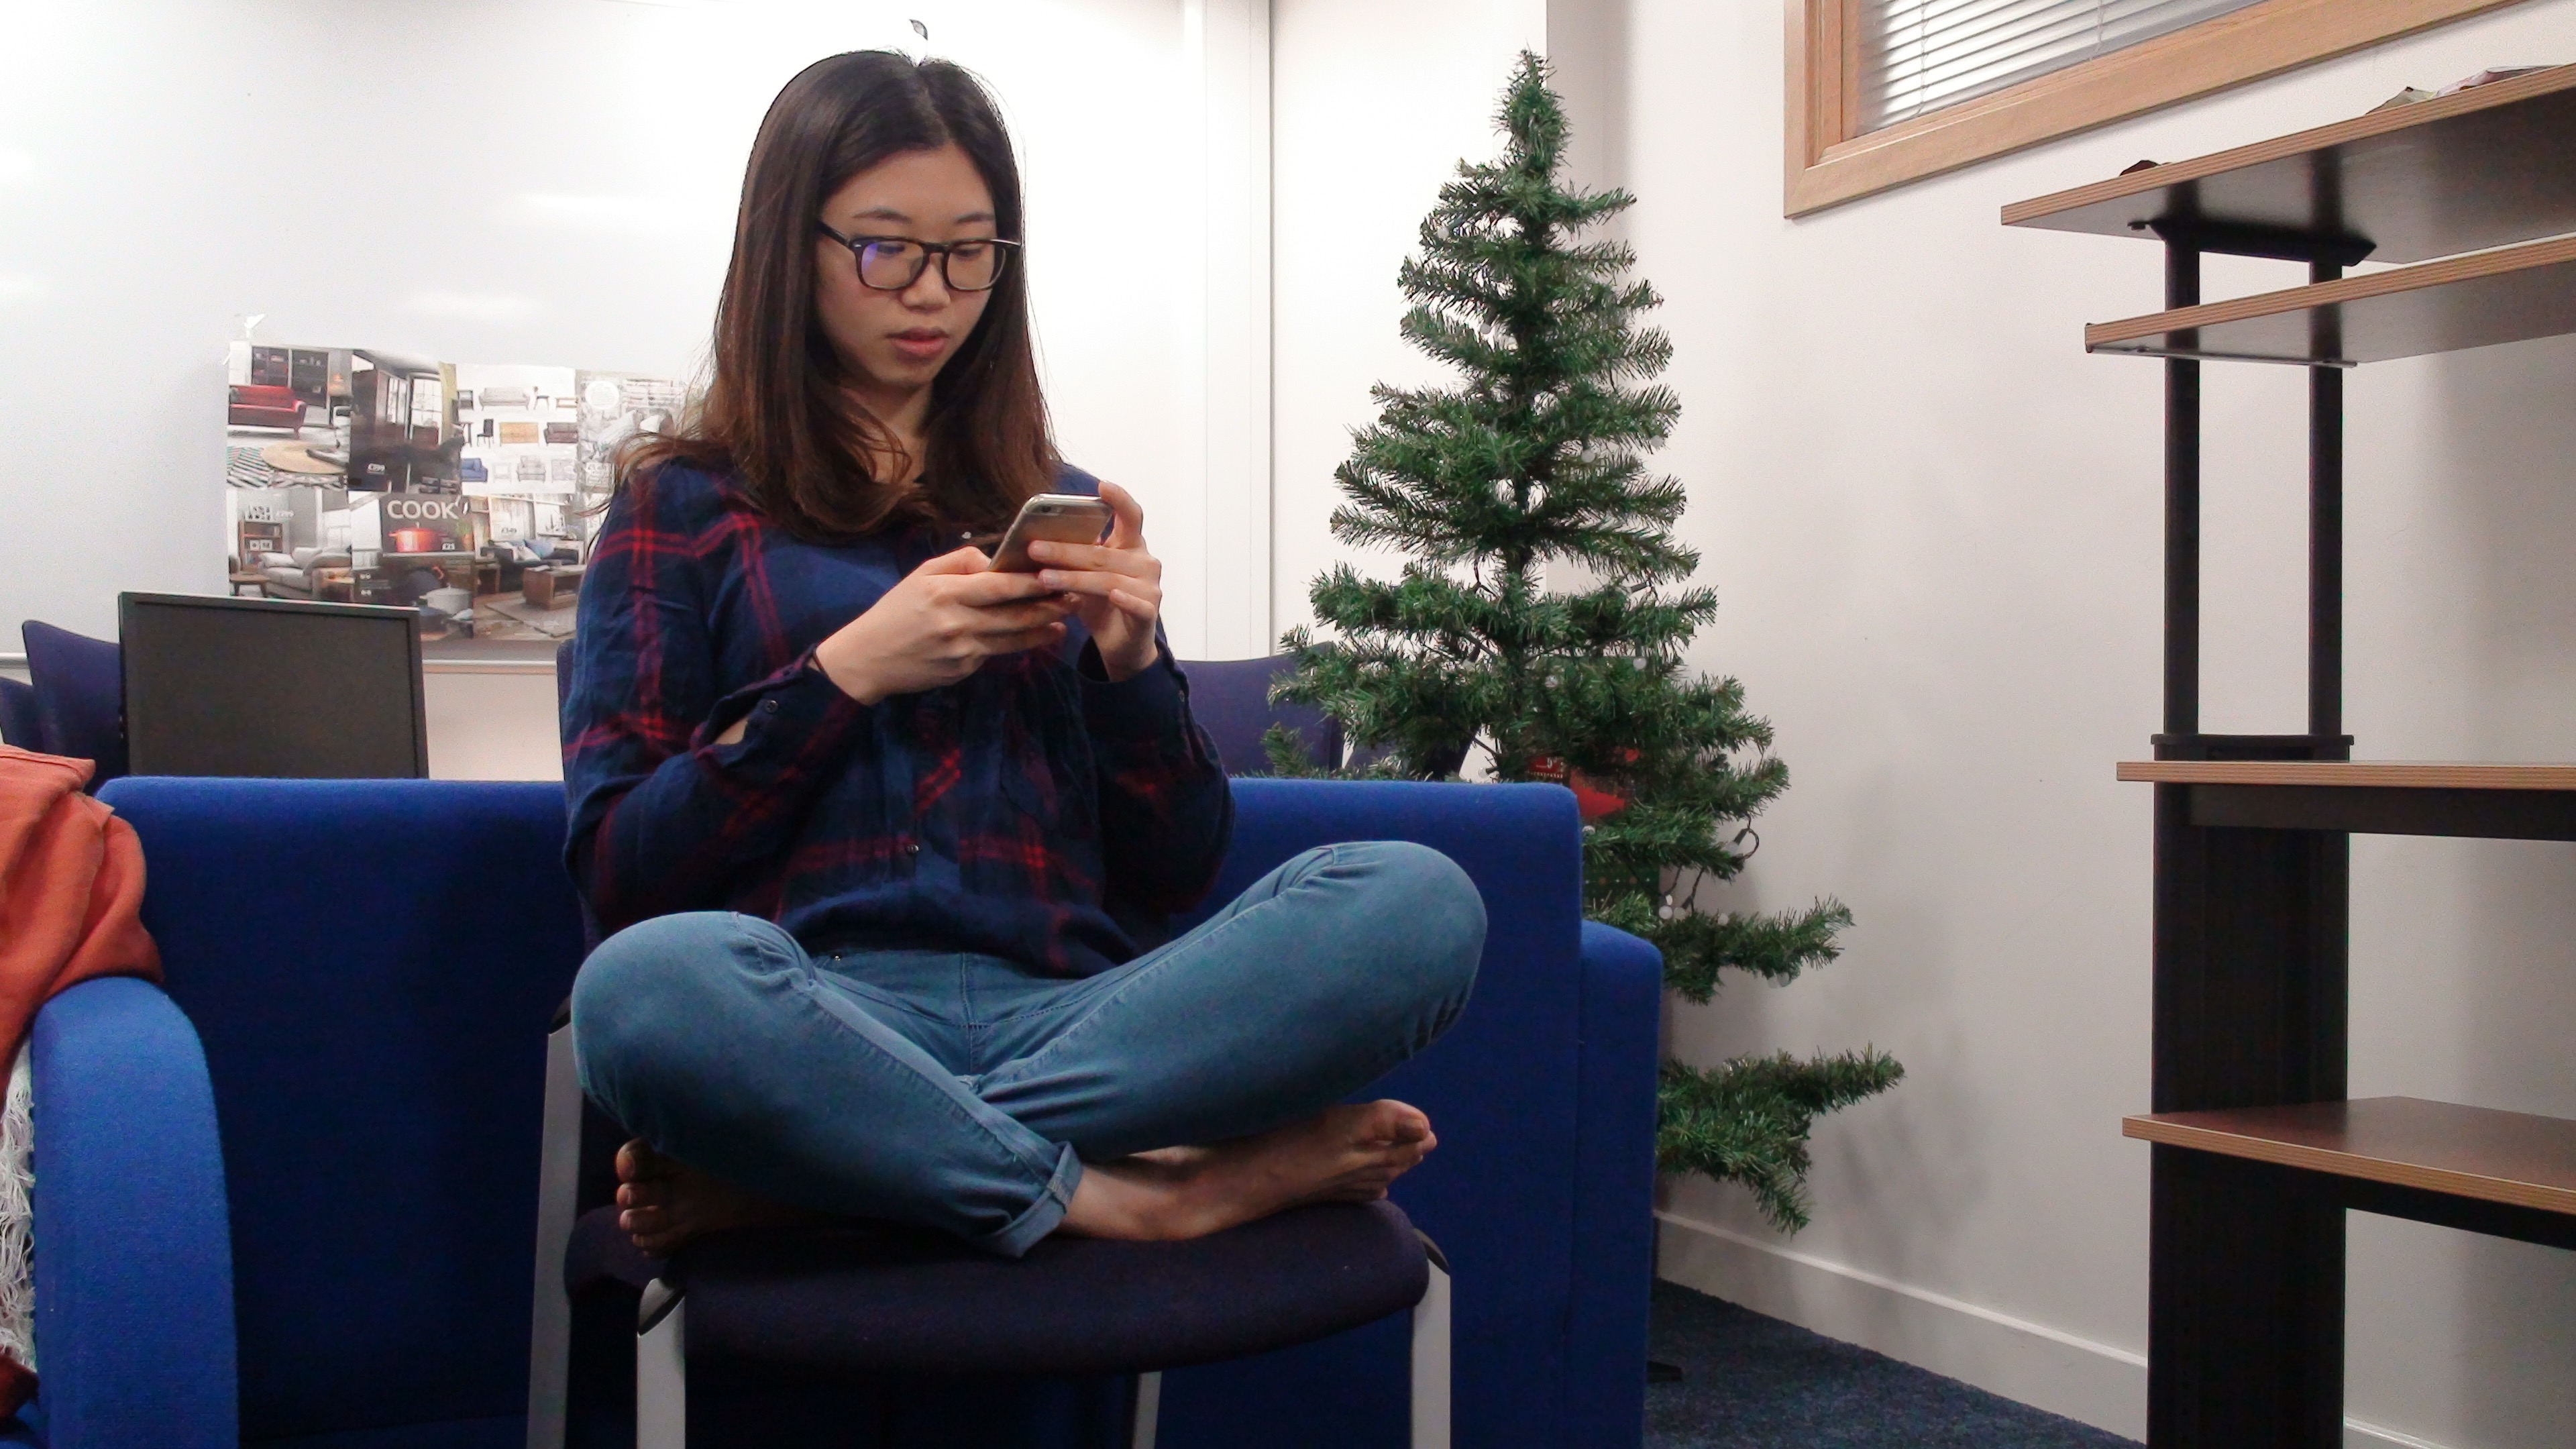
\includegraphics[width=0.5\textwidth]{figs/c3}
    \caption{Leg-Crossed Type 3}
    \end{figure}
  \end{itemize}

  \item lower back not supported \hfill \\
  \[ Z of SpineMid- Z of SpineBase > d\]
  \[ AND\]
  \[ Y of SpineShoulder - Y of SpineBase < e\]
  \begin{figure}[h]
  \centering
    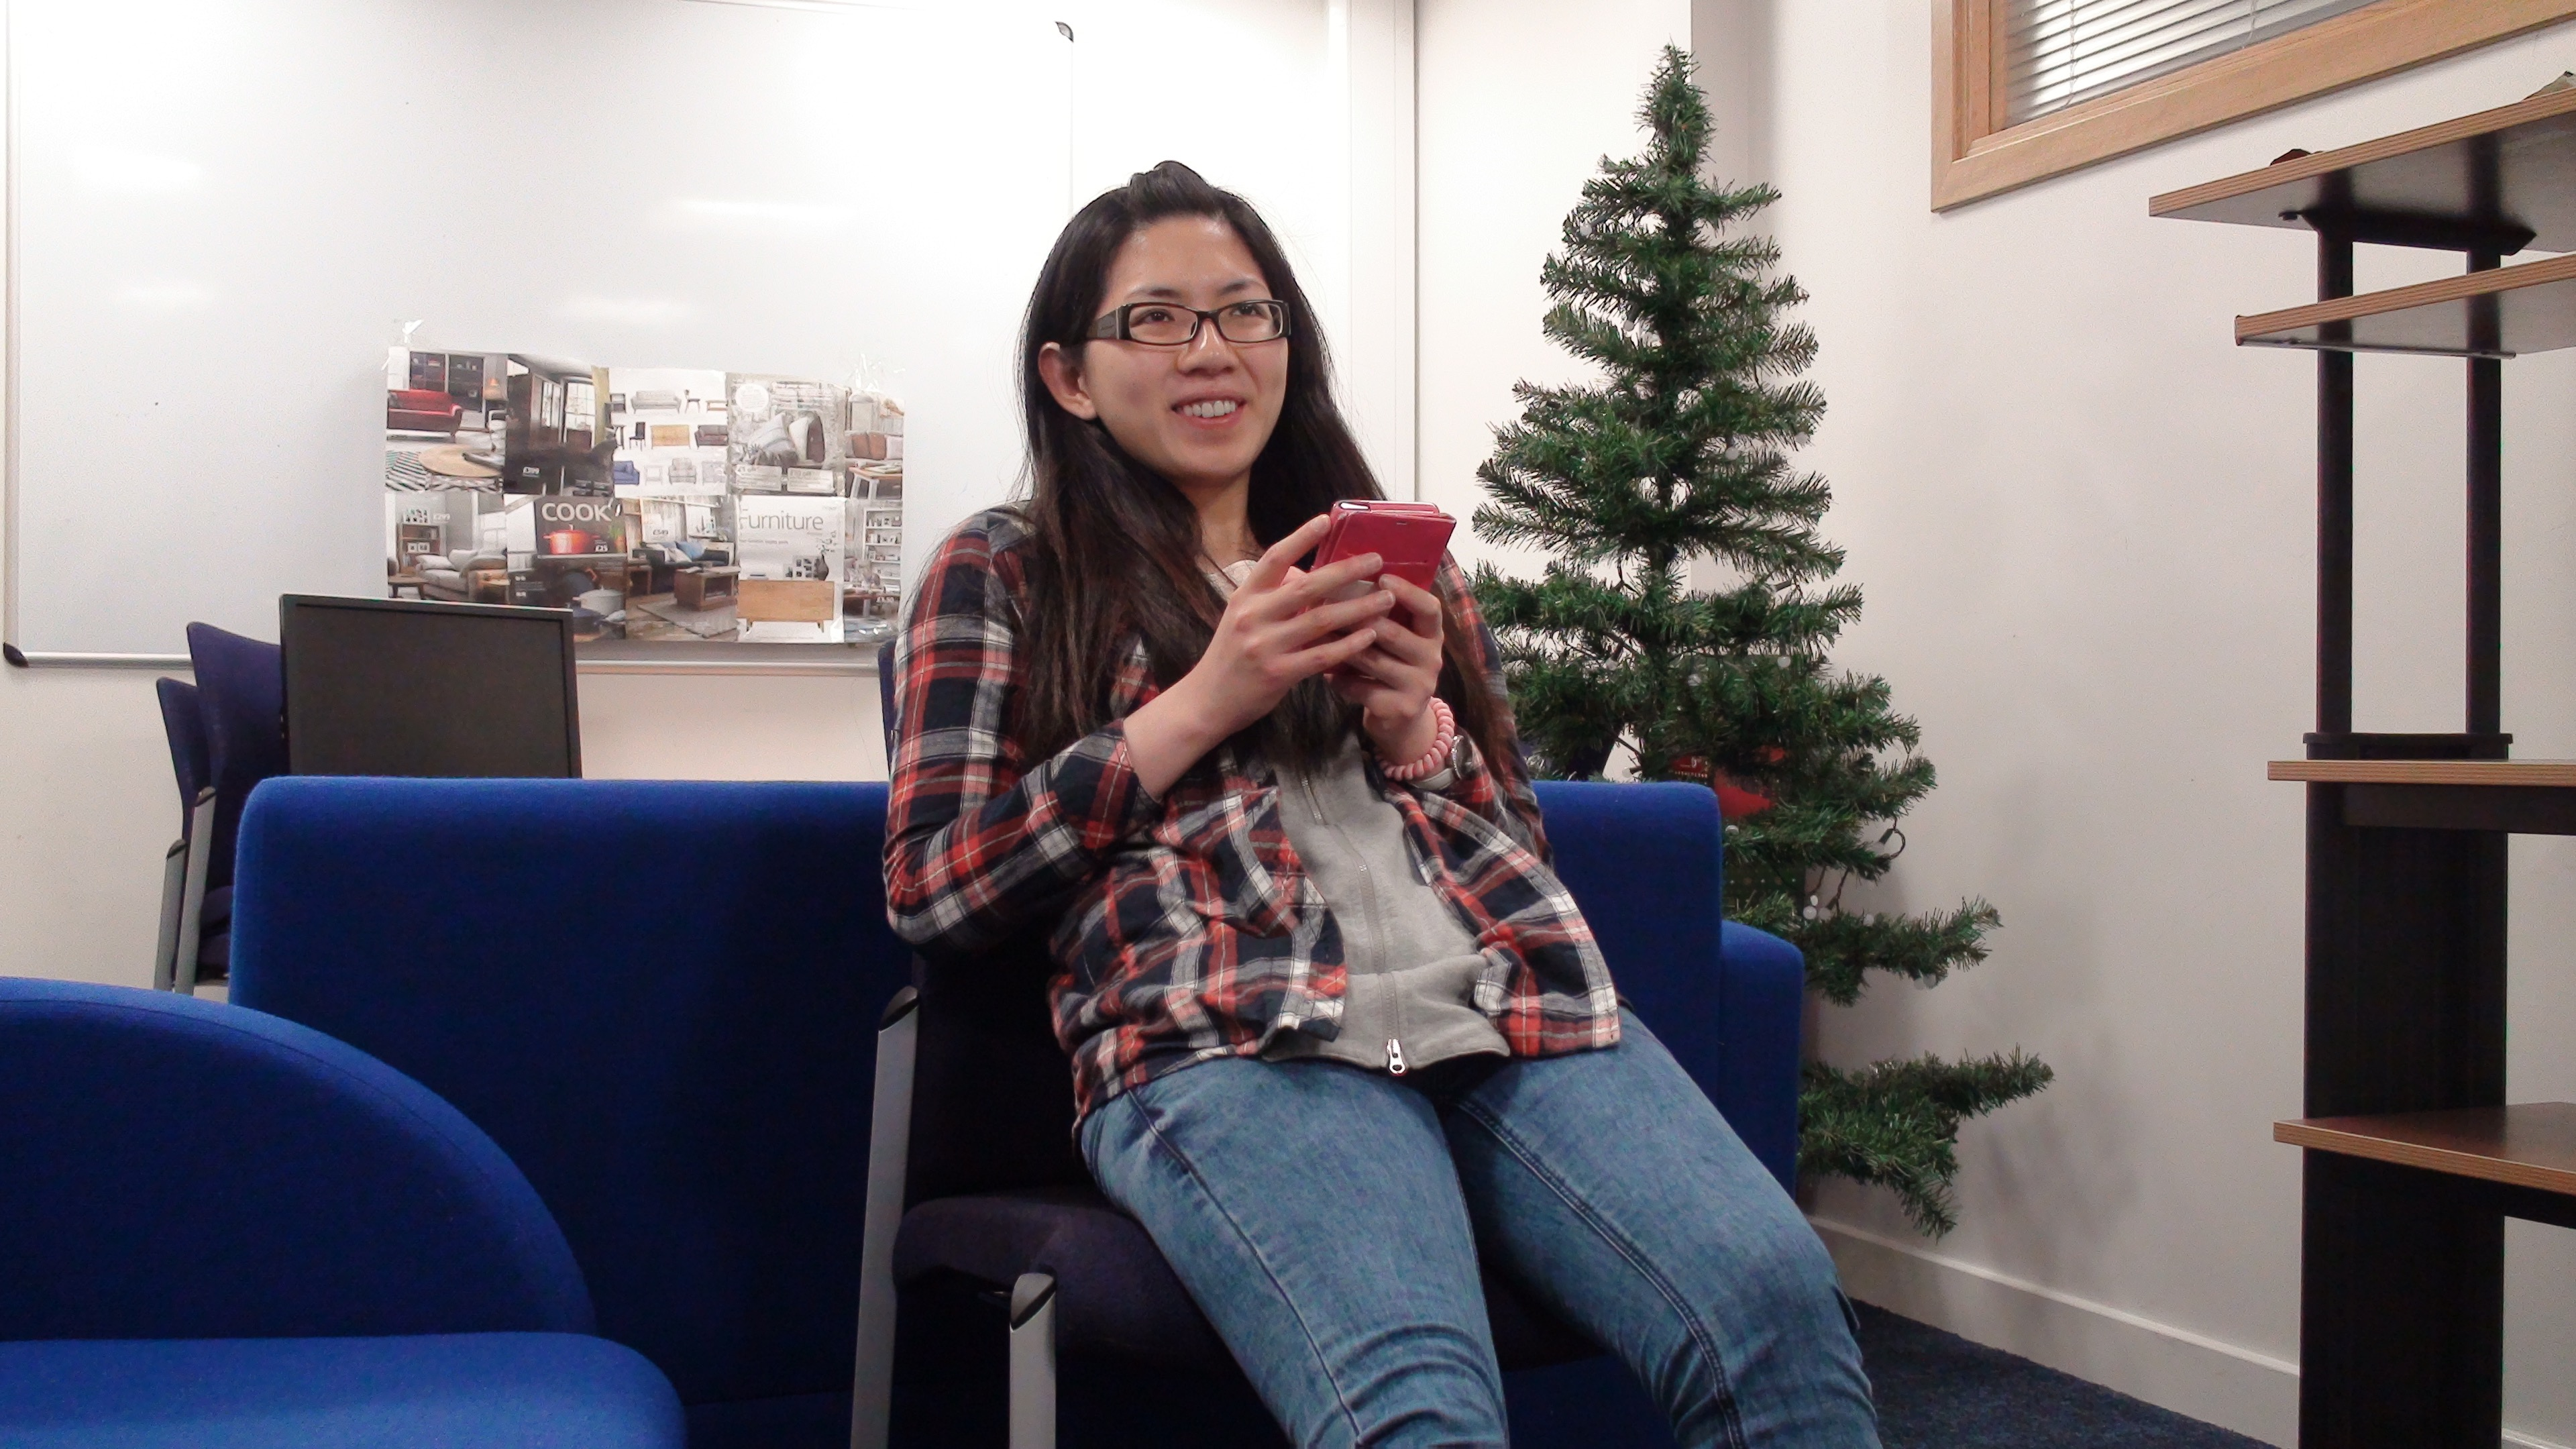
\includegraphics[width=0.5\textwidth]{figs/l1}
  \caption{Lower-Back Not Supported}
  \end{figure}

  *The formula used to classify the lower-back-not-supported posture can adopt position Z of the joints to be its variables, because having this posture should be sitting against the back of sofa and the problem of body orientation should not exist in this condition.

  \item slouch \hfill \\
  \[( Z of SpineMid - Z of SpineBase )*(Z of SpineMid - Z of SpineShoulder )  > 0\]
  \[OR\]
  \[( X of SpineMid - X of SpineBase )*(X of SpineMid - X of SpineShoulder )  > 0\]
  \[OR\]
  \[ Distance(PositionLeftShoulder - PositionLeftHip)< f\]

  \begin{figure}[h]
  \centering
    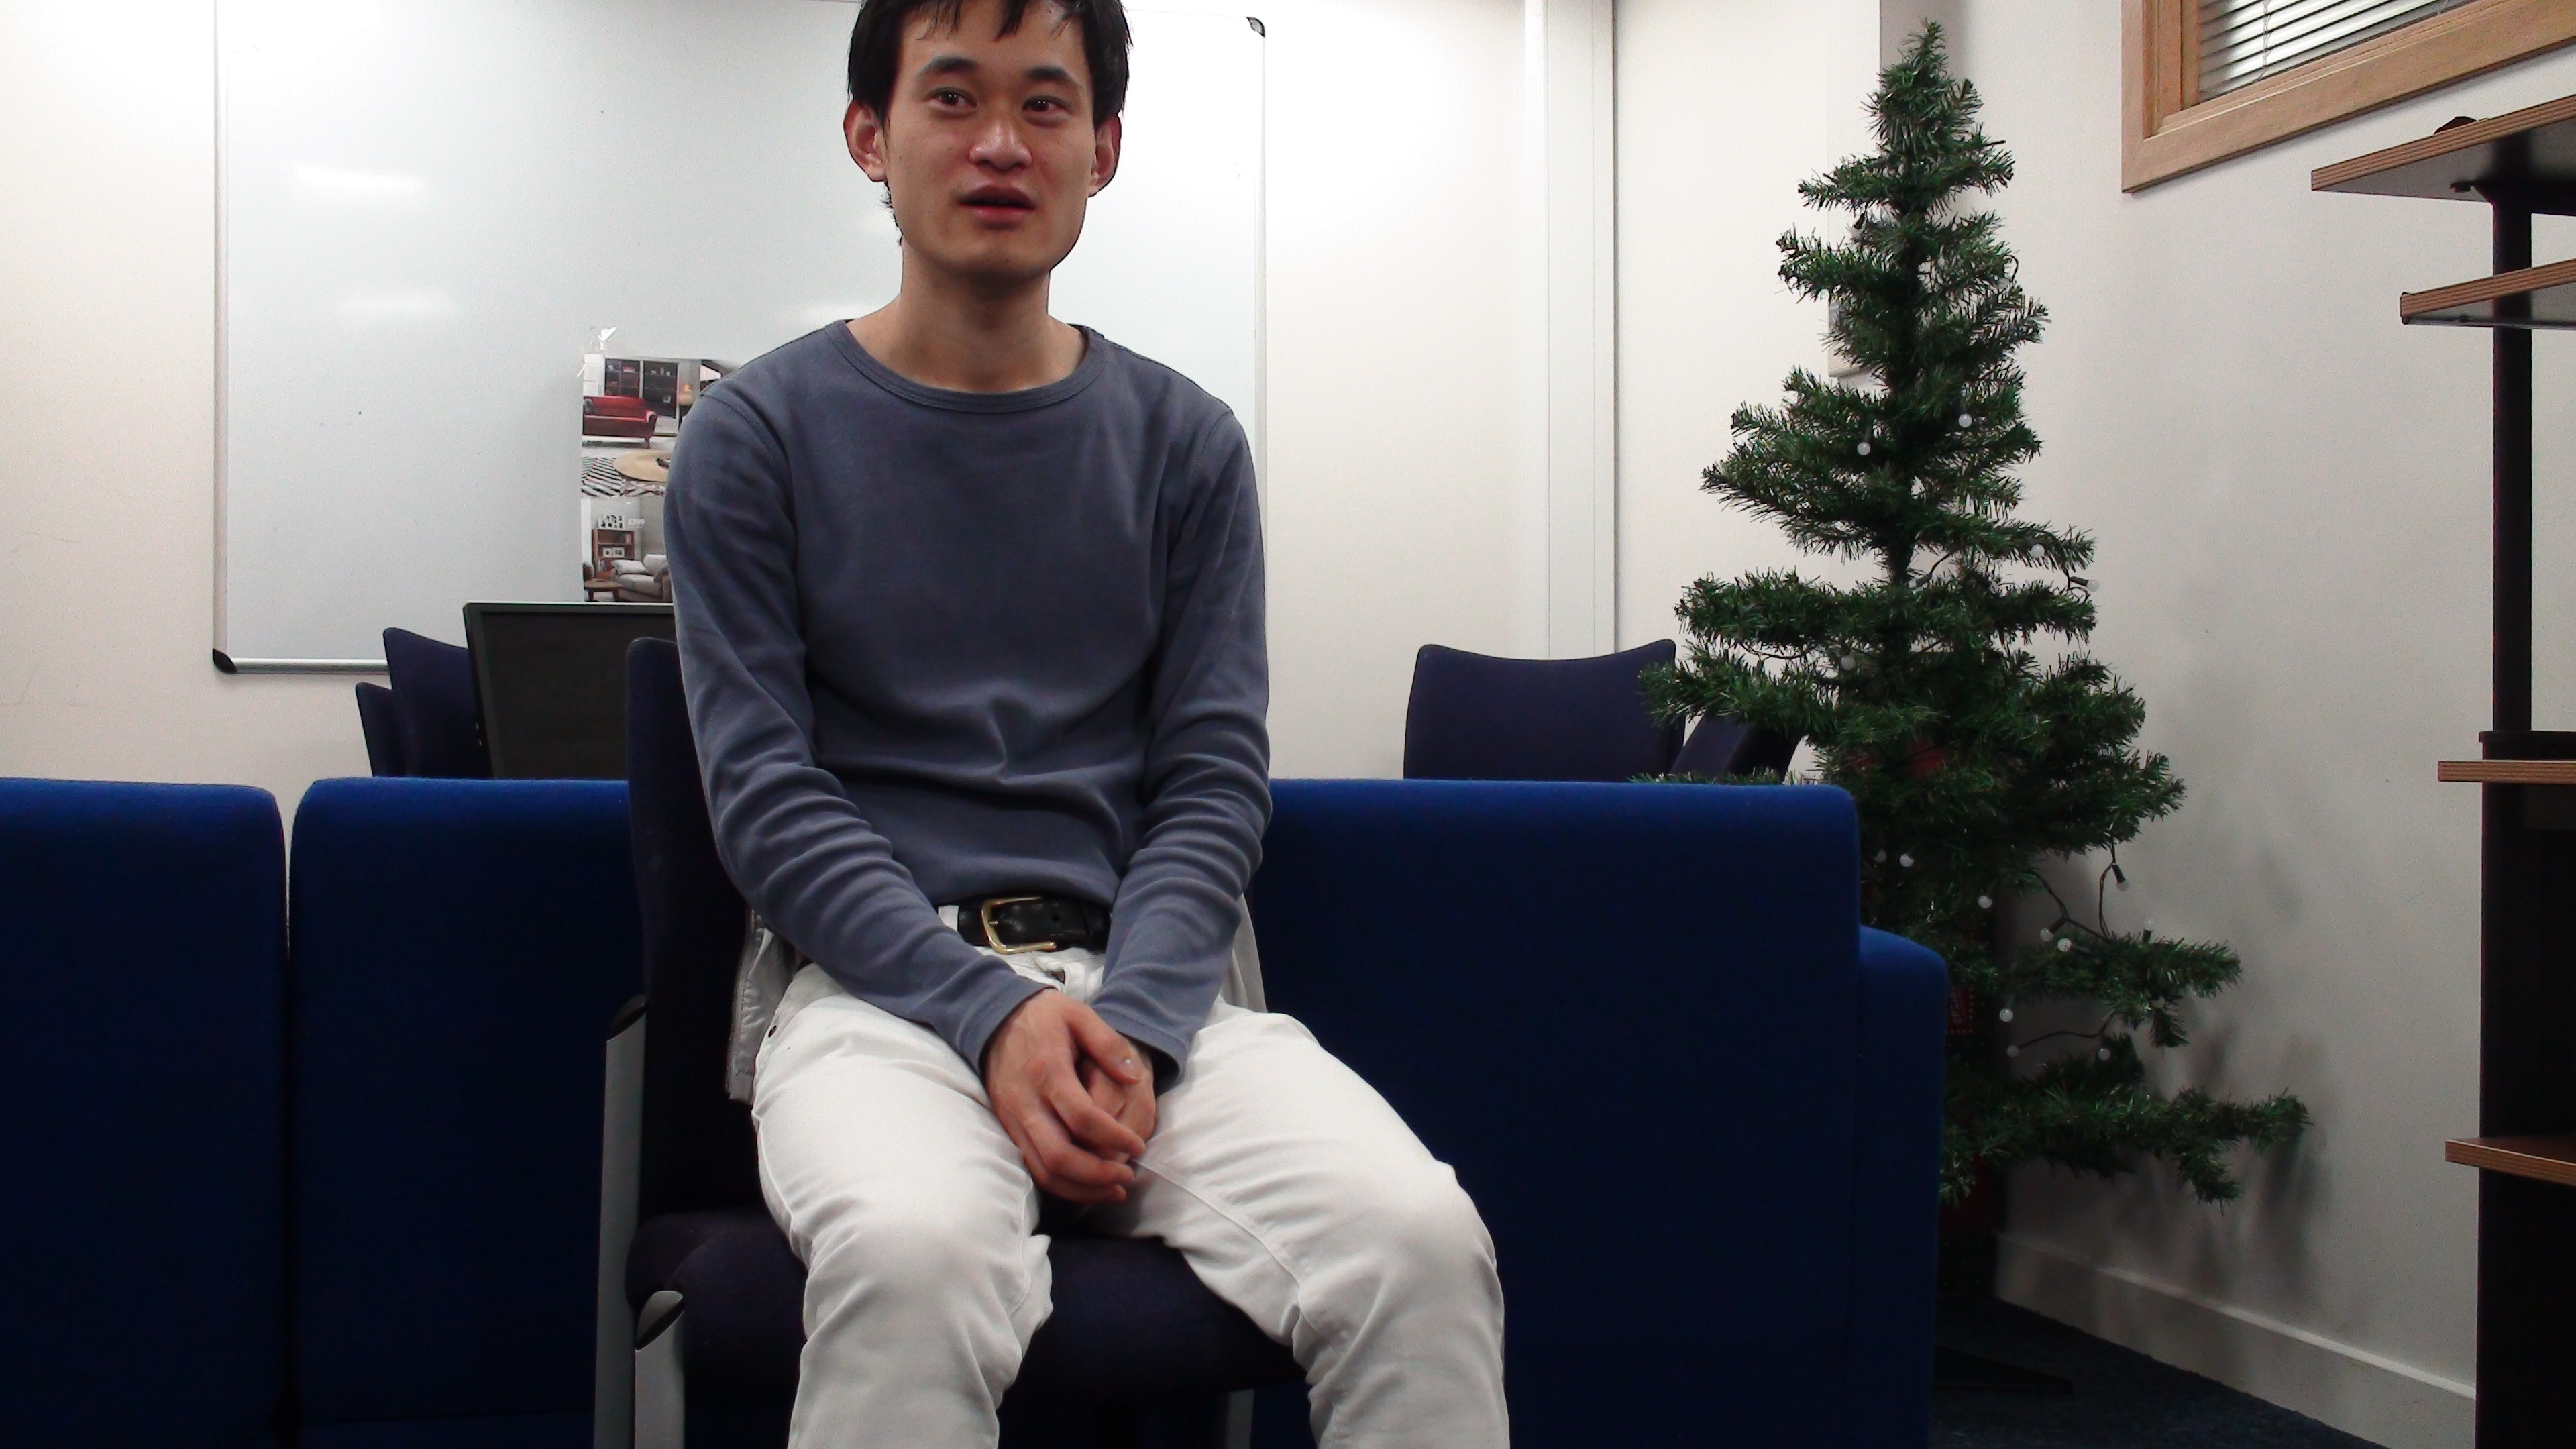
\includegraphics[width=0.5\textwidth]{figs/s1}
  \caption{Slouch}
  \end{figure}

  \item stationary \hfill \\
  *Clean the outliers of the data collected from the stationary posture measurement, and calculate the variance for each joints to define the 99.5 percent confidence interval that the values may vary.
  \item viewing height
  \begin{itemize}
    \item low viewing height
    \[ Y of Head - Y of Neck < g\]
    \[ AND\]
    \[ (Z of Neck - Z of Head > h ) || ( X of Head - X of Neck > i)\]
    \item high viewing height
    \[Y of Head - Y of Neck > j\]
    \[ AND\]
    \[ (Z of Head- Z of Neck > k ) || (X of Neck- X of Head > l)\]
    \begin{figure}[h]
    \centering
      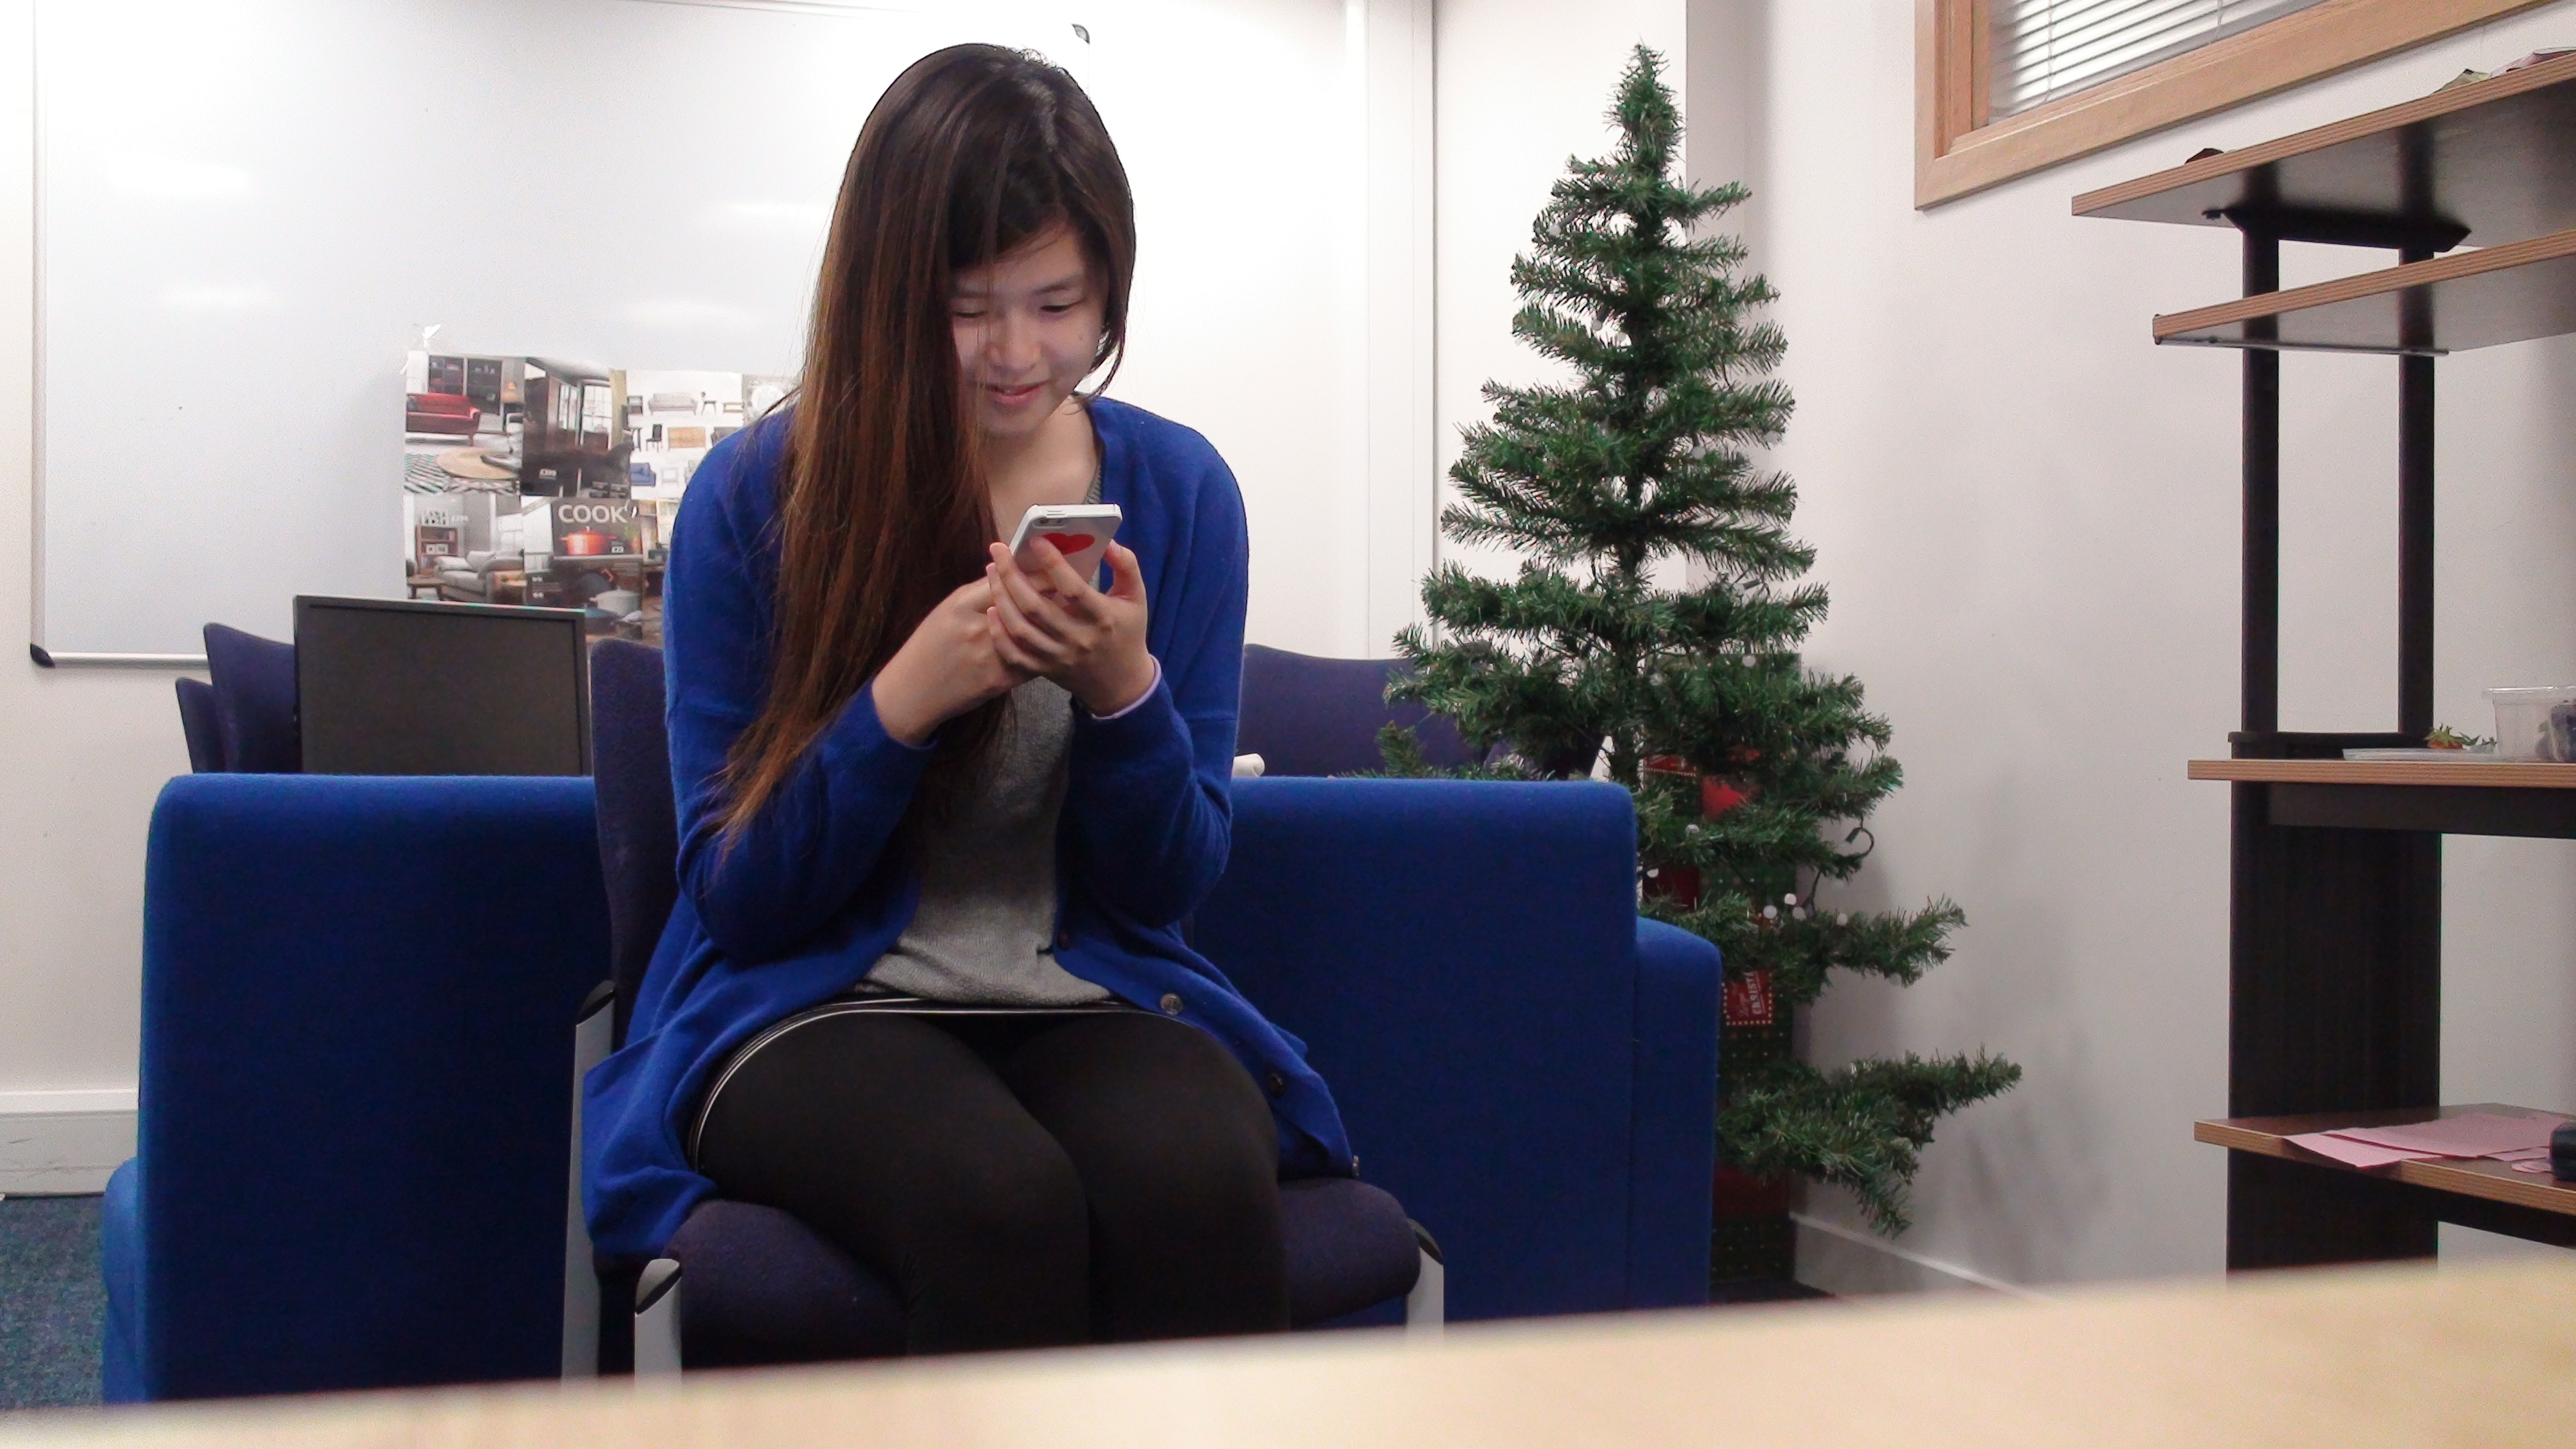
\includegraphics[width=0.5\textwidth]{figs/lh1}
    \caption{Low Viewing Height}
    \end{figure}
  \end{itemize}
\end{enumerate}

\subsection{Priority of Posture Feedback}
The regulation priority among the target postures is determined by both subjective reports in section one and objective observations in section two. The subjective factors include the degrees of relax and the sense of body comfort to each posture. The value of the body comfort is calculated by averaging the degrees of neck, shoulder, and spine comfort, which are investigated along with the degrees of relax after a subject has had a specific posture for the given time using the Likert 5 points scale. The result is summarized in figure 3. The patterns of relax and body comfort follow a similar trend. The participants reported the highest relax score (4.41) after having a stationary posture for 3 minutes, followed by the leg-crossed (4.25) and the lower-back-not-supported (4.25). The participants felt relatively not relax after having standard (3.75) and slouch (3.75) postures. As for body comfort scores, both stationary and leg-crossed postures are ranked in the first place (3.86), while the lower-back-not-supported in the second place (3.64), and the standard in the third place (3.61). The slouch posture (3.44) is rated as the least comfortable posture among the five.The patterns of degrees of relax and degrees of body comfort to the target postures follow a similar trend.

\begin{figure}[h]
\centering
  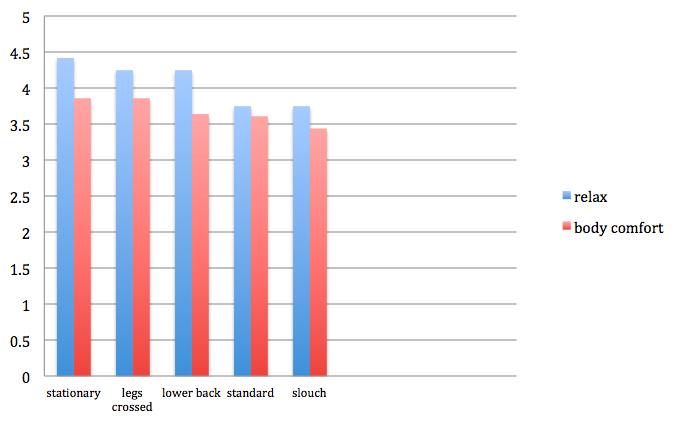
\includegraphics[width=0.5\textwidth]{figs/subjective}
\caption{The degrees of relax and body comfort to each posture}
\end{figure}

According to the subjective data alone, the slouch could be the top priority of our behavior regulation, as the lower degrees of comfort might indicate the higher risk to body injury. Based on this assumption, the order of the regulation followed the slouch should be lower-back-not-supported, leg-crossed, and stationary. However, the higher degrees of body comfort and relax could also indicate the measured posture is more frequently had by a subject. The assumption is supported by the fact that the standard posture, which should be the most appropriate and healthy one among the five, is only ranked at the fourth place with regard to the sense of relax and comfort of the participants. The participants might feel less comfortable when having a standard posture rather than a leg-crossed one, a lower-back-not-supported-one, or a stationary one because their bodies are not used to having such postures. The fact again proves the seriousness of the bad-posture issue.If the second assumption were true, the order of the posture regulation would be stationary, leg-crossed, lower-back-not-supported, and slouch. The analysis of the scenario study could help to determine the more reasonable assumption.

\subsection{Feedback Specification}

\subsubsection{Incentives}
Understanding the incentives for the users to improve their postures can be helpful in the feedback system design. The participants mentioned having better body shape, protecting eyes, becoming healthier, and feeling more comfortable as the main attracting points for them to improve their postures. 25 percent of them presented that seeing the research of an expert indicating the impact of bad postures would increase their willingness to improve their postures. Some participants from the 25 percent also mentioned that the knowledge from the research should be demonstrated using clear diagrams rather than lots of words. This might reflect the explanation path that the users' are convinced about the importance of having good postures could be a peripheral one. When taking a peripheral route, the user's' judgements would more likely be influenced by the source of information, humor, sexual hints, fear, and positive emotion (Petty and Cacioppo, 1986). Therefore, the system could deliver the feedback to a detected posture using the information from a credible source, or presenting the feedback in a way which makes people happy or exciting. Using the fear as a technique would not be considered because a positive user experience is emphasised.

The further investigation on the importance of different factors related to the posture improvement shows that the most critical reasons for posture improvement is owning a better body shape (37 percent), followed by becoming healthier (25 percent) and avoiding discomfort (25 percent), then is the last one, avoiding fatigue (13 percent). This could be explained by the assumption that the driving forces of having good postures (62 percent) might be stronger than the pushing force of avoiding bad postures (38 percent) on this issue. The assumption could be applied on the feedback system design such as using the techniques of positive reinforcements rather than the techniques of negative reinforcements. However, even though avoiding discomfort is classified as a pushing force, its high rating score still indicates the high concerns from the users and should not be ignored.

\begin{figure}[h]
\centering
  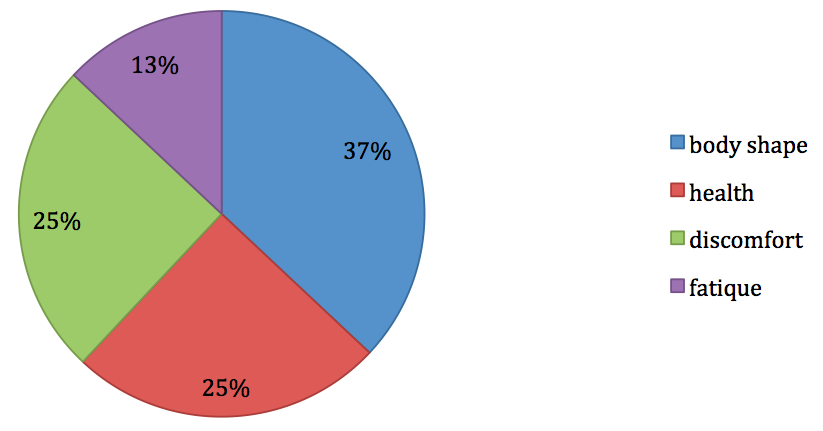
\includegraphics[width=0.5\textwidth]{figs/importance}
\caption{importance of incentives for having good postures}
\end{figure}

\subsubsection{Feedback methods}

There are five feedback methods to be compared with regard to the efficiency belief and the preference respectively. The candidates include simply presenting the current posture, presenting the current posture by a funny way, presenting the current posture by a cool or novel way, showing the impact of current posture, and providing compliments when the users are having good postures. The result of the investigation is illustrated in figure 4.6, as showing the impact of current postures is believed to be most effective, while receiving compliments for the good postures as well as knowing the impact of bad postures are most preferred. Providing compliments to good postures is highly ranked in both efficiency regard and preference regard, which means the feedback for improving the postures would not only help when bad postures show, but also when good postures does.

The result might also indicate that an informative feedback could be better recommended than a non-informative one, because showing the impact of current postures is apparently more informative than the others. The way to present the impact of current posture can be further discussed, however, the ranking of the methods to illustrate current posture could be analogous to the ways to demonstrate the impact of current postures. Namely, a cool/ novel way is slightly better than a cute/funny way, and the two are rated greatly higher than a simple way. Using a cool/novel way to show the impact of current posture is therefore identified as the most useful feedback methods based on the study.

\begin{figure}[h]
\centering
  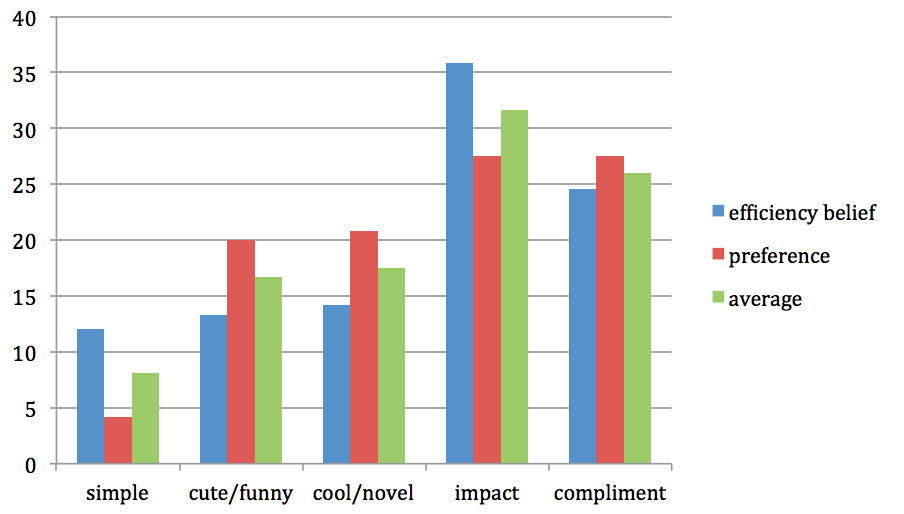
\includegraphics[width=0.5\textwidth]{figs/method}
\caption{Attitudes to feedback methods}
\end{figure}

\subsubsection{Feedback channels}
The posture feedback can be delivered within different perceptual channels among visual, audio, or touch. The audio channel is believed to be the most effective one, but its preference is just slightly higher than the visual channel, while the touch channel is significantly less identified with regard to both the efficiency belief and the preference. The difference of average scores between the audio and the visual channels should mainly contribute to the efficiency belief. However, such a strong efficiency belief for the audio channel could come from the property of an audio message, which is generally obtrusive. Due to this premise, the user experience design for applying audio feedback should be particularly considered.

\begin{figure}[h]
\centering
  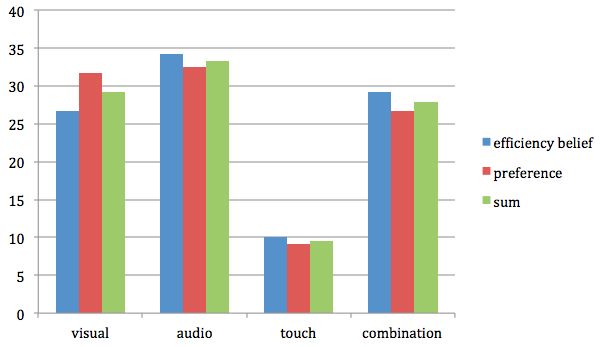
\includegraphics[width=0.5\textwidth]{figs/channels}
\caption{Attitudes to feedback channels}
\end{figure}

\begin{figure}[h]
\centering
  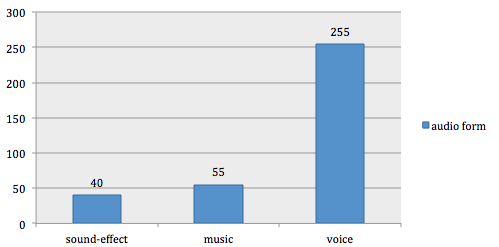
\includegraphics[width=0.5\textwidth]{figs/audioform}
\caption{Weighting for audio forms}
\end{figure}

The diagram of different audio forms shows the weighting value of the chosen audio form of each participant by their average ratings to efficiency belief and the preference for audio channel. Voice is rated as the most useful form, intensively higher than the other. Music is also graded over sound effect. This could also be contributed to the informative property as the analysis of feedback methods suggests.

The combination is generally defined as visual plus audio or all the three together. Interestingly, although the combination of using multiple channels is believed to be very effective, its preference is at least 10 percent lower than the visual and the audio. This might indicate the worry for the users to receive too complex information at once.

\subsubsection{Others}
The interview also investigated the actions that the participants have adopted for posture improvement. 66.67 percent of the participants said they never use any particular method to improve their posture. However, 37.5 percent of them said that they would remind themselves to avoid some postures, and 12.5 percent of them were given a kind of wearable equipment by their parents to avoid slouch in the childhood; All of them reported no effect for these. 8.33 percent of the participants indicated that they tried doing yoga for the purpose of improving postures, and it did enhance their posture awareness for half year, but the effect faded away when the participants stopped doing yoga. Another 8.33 percent of the participants said they could adjust the chair to make having a good posture more easily. Still 8.33 percent of the participants presented that they would ask themselves to decrease the usage the devices with visual displays and get away from the sofa, as the sofa is somewhere easily make people too relax and have bad postures. The other 8.33 percent of the participants claimed they would ask themselves to stand against a wall and this is helpful for them to remember the feeling of keeping the spine straight. The information of these methods could be provided if the suggestions for posture improvement are required by the feedback system.
